\begin{figure}[!p]
\centering
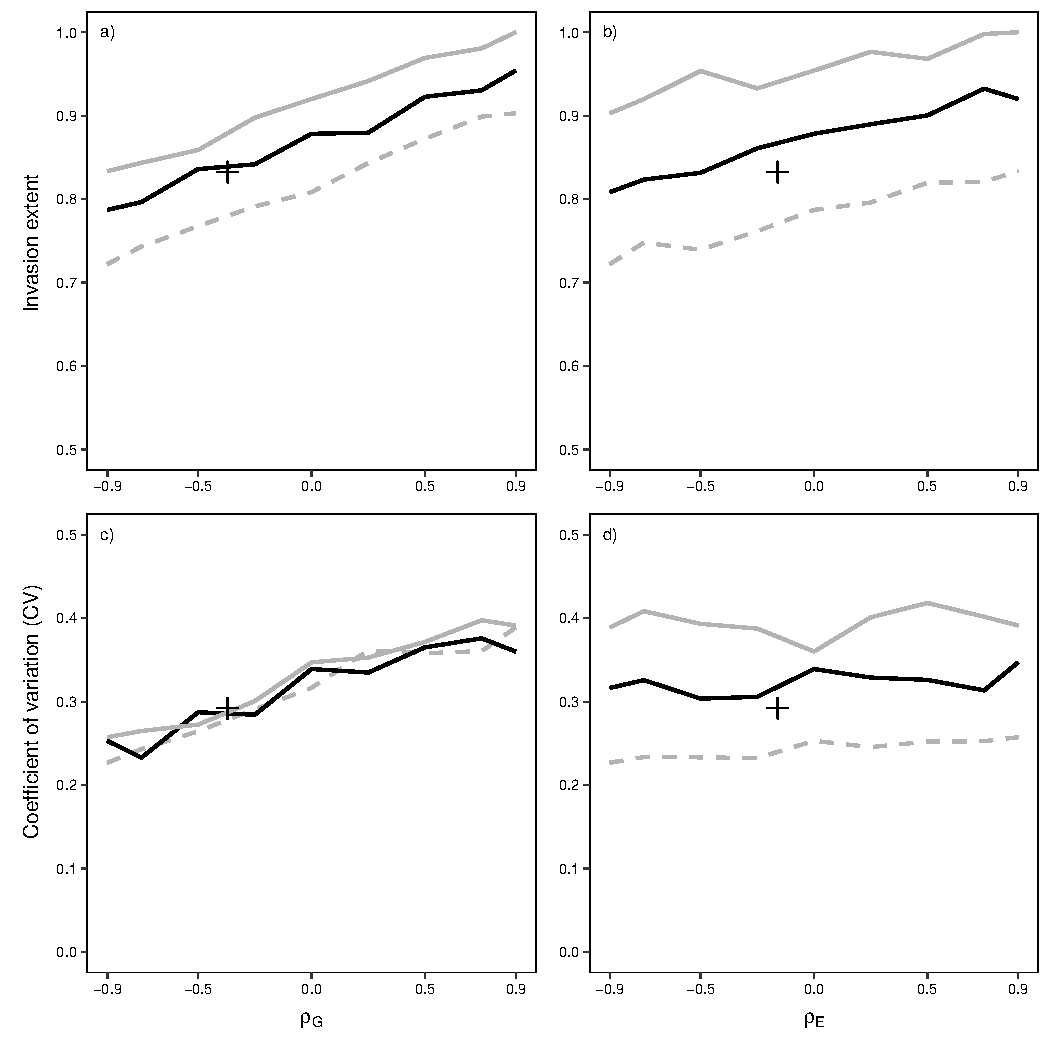
\includegraphics[width=0.95\linewidth]{Figures/corr_extent_and_CV.pdf}
\caption[Mean and coefficient of variation (CV) in invasion extent]
{\textbf{Mean and coefficient of variation (CV) in invasion extent.} Panels a) and c) show varying $\rho_{G}$ on the x-axis with each line representing a different level of $\rho_{E}$: 0.9 (solid, gray), 0 (solid, black) and -0.9 (dashed, gray). Panels b) and d) show varying $\rho_{E}$ on the x-axis with each line representing a different level of $\rho_{G}$: 0.9 (solid, gray), 0 (solid, black) and -0.9 (dashed, gray). The $\bm{+}$ symbol on each plot indicates the values that correspond directly to the \textit{C. maculatus} system ($\rho_{G}$ = -0.37, $\rho_{E}$ = -0.16). In panels a) and b), the y-axis is scaled relative to the largest value, so that so that the greatest simulated mean invasion extent corresponds to a value of 1, and other invasion extents are reported relative to that value.} \label{corr:extent} \end{figure}